%scrrprt ist eine Klasse für Berichte und längere Arbeiten
\documentclass[11pt,a4paper]{scrreprt}
%ermöglicht die Eingabe von Umlauten usw. ohne Codierung
\usepackage[utf8]{inputenc}
%Schriften werden mit einer passenden Kodierung für europäische Zeichen ausgegeben
\usepackage[T1]{fontenc}
%Passt Dokumentelemente an die Konventionen der deutschen Sprache (neue Rechtschreibung) an, z.b. Datumsangaben, Silbentrennung
\usepackage[ngerman]{babel}
%Grafikpaket
\usepackage{graphicx}
\title{Lastenheft}
\author{Lisa Vogelsberg}
\date{29.11.2017}

\begin{document}
\tableofcontents

%Bei reports beginnt die Zählung von sections mit 0. Daher wurde hier chapter gewählt. Danach kann section gewählt werden, danach subsection und subsubsection
\chapter{Ausgangssituation}
%LV: Übernommen aus der Themenbeschreibung im OLAT
Schon seit langer Zeit gilt die Devise: Wissen ist Macht. Daran hat sich auch im 21. Jahrhundert nichts geändert. Aus diesem Grund ist die Adaption von neuem Wissen unumgänglich, jedoch ist der Weg dahin meist nicht der Erfreulichste: Das Aneignen von Wissen wird meist mit Lesen, auswendig Lernen und ständigem Wiederholen in Verbindung gebracht und ist dementsprechend bei einem Großteil der Bevölkerung negativ konnotiert. Wissen lässt sich aber durchaus auch 'spielerisch' aneignen, etwa wie dies kleine Kinder völlig unbewusst tun.\\
An diesem Punkt kommen die Wissenspiele zur Sprache. Für den privaten Gebrauch gibt es bereits viele, gut funktionierende, Ansätze, z.B Spiele wie Quizduell oder Fernsehshows wie "Wer wird Millionär". Für die betriebliche Weiterbildung, also Erschließung neuen Wissens innerhalb von Unternehmen, gibt es jedoch bisher nur wenig Anwendung solcher Ansätze. Das Institut für Angewandte Informatik der Universität Leipzig erprobt und erforscht zur Zeit im Rahmen des Projekts SB:Digital (http://sbdigital.infai.org/) gamifizierte Prozesse des Lernens.
Das erhebliche Potenzial von Wissensspielen hat sich diesbezüglich bereits erwiesen. Angeknüpft an diese Forschungsergebnisse soll im Rahmen dieses Projektes ein gamifiziertes Wissenquiz zur Verwendung innerhalb von Unternehmen entstehen.
\chapter{Zielsetzung und Produkteinsatz}
\section{Vision}
%LV: Ich krieg das nicht schön bzw. prägnant ausformuliert, deswegen erstmal so. Vielleicht kann das jemand besser ausdrücken.
Mitarbeiter von Unternehmen sollen mit Hilfe des entstehenden Quiz weitergebildet werden. Sinn und Zweck der Anwendung bildet also die Vermittlung von Wissen. Nun könnte dies natürlich per Dekret an die Mitarbeiter getragen werden, sich in Form von Seminaren oder Fortbildungen Wissen anzueignen, jedoch erfreuen sich diese Formen meist nicht der größten Beliebtheit. Aus diesem Grunde soll durch Gamification mit Spaß und Unterhaltung dazu motivieren, selbst aktiv zu werden. Durch das Quiz soll die Wissensvermittlung nicht als Last, sondern als Freude bzw. Spaß empfunden werden. Im besten Fall geht dies so weit, dass sich die Mitarbeiter noch über das notwendige Maß (z.B. in ihrer Freizeit) hinaus an der Weiterbildung beteiligen. 
\section{Zielsetzung}
Die zu entwickelnde Software soll unter Verwendung verschiedener Techniken der Gamification die betriebliche Weiterbildung und den Wissensaustausch unterstützen.
Als Kernkomponente soll ein Quiz mit einer Frage, n Auswahlmöglichkeiten und genau einer richtigen Antwort erstellt werden, an dem Gruppen von mindestens 5 Personen teilnehmen.
Gewinnen soll dabei aber nicht immer nur derjenige, der am meisten weiß, sondern derjenige, der Wissen, Strategie und Zufall für sich zu nutzen weiß.
\section{Produkteinsatz}
Zielgruppe des Produkts sind Arbeitnehmer in Unternehmen verschiedener Branchen, die sich während ihrer Arbeitszeit mit dem Quiz beschäftigen. Die Teilnahme erfolgt dahingehend anonym, dass nicht festgestellt werden kann, welche reale Person gerade an dem Quiz teilnimmt, sofern diese das wünscht.

\chapter{Funktionale Anforderungen}
%LV: Muss- und Kann-Ziele finde ich für die Anforderungen noch nicht ganz passend, da man sie zu schnell mit den Zielen verwechseln die kann, die man vorher festlegt hat und durch die sich dann die Anforderungen ergeben. Einteilung in Hauptanforderungen und optionale Anforderungen trifft es vielleicht schon eher, ist trotzdem noch nicht gut von mir gewählt (Hauptanforderungen meint nämlich eigentlich etwas anderes). Würde ich Dienstag gern besprechen, wenn wir bis dahin nicht noch eine bessere Bezeichnung gefunden haben.
\section{Muss-Ziele}
%Erzeugt eine Liste ohne Nummerierung, bei dem das Wort in eckigen Klammern als Beschreibung dient und fett gedruckt wird. Neue Zeilen innerhalb eines items werden eingerückt.
\subsection{An- und Abmelden}
\begin{description}
\item[/LF0010/] Registrierung \\
Ein Nutzer soll sich unter Angabe eines Nutzernamens, Passworts und E-Mail registrieren können.

\item[/LF0020/] Anmelden \\
Ein Nutzer soll sich mit seinem Nickname und Passwort einloggen können.

\item[/LF0040/] Anzeige der Accountübersicht \\
Nach dem Anmelden kann der Benutzer die Startseite seines Spieler-Accounts einsehen. %Entsprechenden Verweis noch einfügen

\item[/LF0030/] Abmelden \\
Der Nutzer soll sich vom System abmelden können.

\item[/LF0040/] Passwort anfordern \\
Der Nutzer soll sein Passwort anfordern können, wenn er dieses vergessen hat.

%Falscher Ort für das Profil
\item[/LF0050/] Spielerprofil \\
Für jeden Nutzer soll ein persönliches Profil existieren, dass mindestens den Name enthält
\end{description}

% Hier können noch weitere Anforderungen folgen, die mit Einstellungen des Users zutun haben (Privatssphäre, Profil, ...)
\subsection{Spieleraccount}
\begin{description}
\item[/LF0110/] Account Details \\
Über den Account sollen folgende Informationen eingesehen werden können
	\begin{itemize}
	\item Angemeldeter Benutzername
	\item Angemeldete E-Mail
	\item Registrierungsdatum
	\end{itemize}
	
\item[/LF0120/] Änderung des Passworts \\
Ein Benutzer soll sein Passwort beliebig häufig ändern können.

\item[/LF0130/] Löschung des Accounts \\
Der Benutzer soll selbstständig seinen Account wieder löschen können.
\end{description}
\subsection{Quiz}

\subsubsection{Rahmen}
\begin{description}
\item[/LF0060/] Fragenpool \\
Es muss ein Pool an Fragen zu einem Thema vorhanden ein, aus dem für das Quiz Fragen entnommen werden können.

\item[/LF0070/] Quizrunde \\
Jede Quizrunde soll dynamisch aus * Fragen zusammengestellt werden.

\item[/LF0080/] Antwort auswählen \\
Der Spieler soll aus n Antwortmöglichkeiten genau eine auswählen können, die richtig ist.
%LV: Die nächste Anforderung muss weitergehend spezifiziert werden bzw. um weitere Anforderungen erweitert werden, was einem zusätzlich noch angezeigt wird oder wann und wie sich ein Score verändert.
\item[/LF0090/]Auswertung einer Frage \\ 
Nach Auswahl einer Antwort soll die Anwendung eine Rückmeldung darüber geben, ob die richtige Antwort gewählt wurde. Falls nicht, so soll die richtige Antwort angezeigt werden

\item[/LF0090/]Anzeige des Punktestands einer Quizrunde \\ 
Der User muss während der Quizrunde jederzeit seinen aktuellen Punktestand sehen können.

\item[/LF0100/] Ergebnisse ausgeben \\
Am Ende einer Quizrunde soll eine zusammenfassende Ausgabe der Ergebnisse erfolgen. Ergebnisse sind: Punktestand eines jeden Teilnehmers (nur die eigene Punktzahl),  individuelle Platzierung als anonymisiertes Leaderboard, d.h. es werden nur die Punktestände angezeigt, sodass jeder nur seine eigene Platzierung aus dem Leaderboard ablesen kann, nicht aber die Platzierungen seiner Mitspieler.

\item[/LF0110/] Dauer einer Quizrunde \\
 Die Dauer einer Quizrunde ist intern, vom Administrator, einstellbar. Sie gilt dann für alle Spiele.
\end{description}

\subsubsection{Spielablauf einer Runde}
Der Spielablauf ist in der Grafik \ref{img:Spielablauf} auf Seite \pageref{img:Spielablauf} verdeutlicht.
Ein Spiel beginnt mit mindestens 5 Teilnehmern. Jeder Spieler der Gruppe erhält die gleiche Frage. Beantwortet er diese Frage korrekt, so erhält er die zu Frage zugehörige Punktzahl auf sein Konto. Wird sie falsch beantwortet, so wandern die Punkte in einen Jackpot. Der Punktwert der Frage wird von ihrer Schwierigkeit beeinflusst (schwere Fragen bringen viele Punkte, leichtere Fragen dementsprechend weniger). Es kann durch Zufall eine Jackpot-Frage ausgelöst werden, in welcher um alle Punkte aus dem Jackpot gespielt wird. Die Jackpot-Frage ist von außen \textit{nicht} von den anderen Fragen zu unterscheiden. Jeder, der die Jackpot-Frage richtig beantwortet, hat Garantie auf einen Anteil des Jackpots. Dieser Anteil wird anhand der Schnelligkeit der gegebenen Antwort bestimmt (Der Schnellste bekommt den größten Anteil). Mit steigender Fragenanzahl (oder steigender Anzahl an falschen Antworten) erhöht sich die Wahrscheinlichkeit, dass eine Jackpot-Frage auftritt. Die letzte Frage einer Runde ist stets eine Jackpot-Frage. In dieser letzen Runde wird der Jackpot-Punktestand verdoppelt und um diesen gespielt. Als Option ist für die letzte Frage eine stattdesseb eine Schnellraterunde möglich.

%Die Grafik muss auch inhaltlich nochmal angepasst werden. Z.b. ist "Tritt bei" als Verzweigungsanweisung angegeben, obwohl da keine Verzweigung ist. Vielleicht können wir für den Schritt, um den Spielablauf zu zeigen, auch den Start zum Quiz komplett weglassen.
\begin{figure}
	\centering
	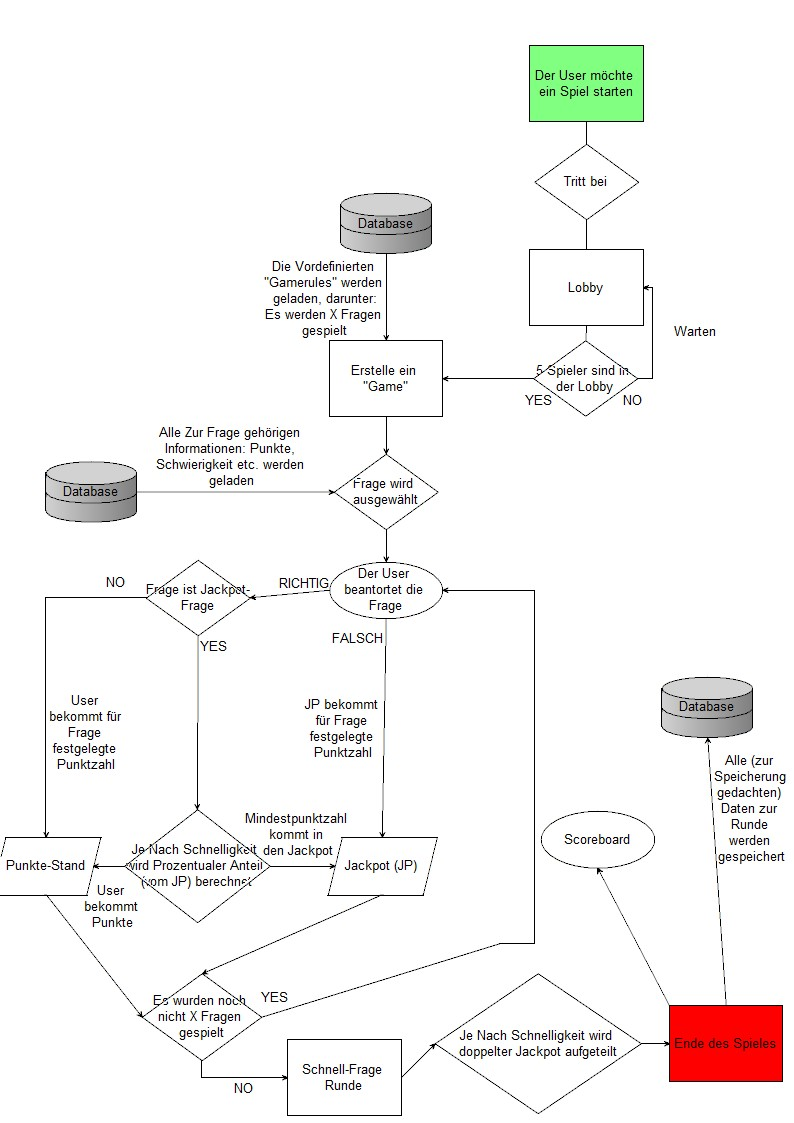
\includegraphics[width=0.9\textwidth, height=0.9\textheight]{Diagramm_002.jpg}
	\caption{Spielablauf als Diagramm}
	\label{img:Spielablauf}
\end{figure}
\begin{description}
\item[/LFXXXX/]Verteilung der Fragen \\
Jeder Spieler der Gruppe soll gleichzeitig die gleiche Frage beantworten müssen.
 
\item[/LFXXXX/]Punkteausschüttung der Frage \\
Wenn eine Frage richtig beantwortet wird, soll der Spieler die zur Frage zugehörige Punktzahl auf sein Konto bekommen, ansonsten gehen die Punkte in einen Jackpot.

\item[/LFXXXX/] Letzte Frage einer Spielrunde \\
Die Anzahl der Punkte des Jackpots in der letzten Frage sollen verdoppelt werden
\end{description}

\subsubsection{Jackpot}
\begin{description}
\item[/LFXXXX/] Ausschüttung des Jackpots \\
Die Punkte des Jackpots können von den Spielern durch Beantwortung einer speziellen Frage (Jackpot-Frage) erhalten werden

\item[/LFXXXX/]Auslösen der Jackpot-Frage \\
Eine Jackpot-Frage soll zufällig ausgelöst werden und sich äußerlich nicht von anderen Fragen unterscheiden.

\item[/LFXXXX/] Auftrittswahrscheinlichkeit einer Jackpot-Frage \\
Mit steigender Fragenanzahl (oder steigender Anzahl an falschen Antworten) soll Wahrscheinlichkeit, dass eine Jackpot-Frage auftritt, steigen. Die letzte Frage einer Runde soll sicher eine Jackpot-Frage sein.

\item[/LFXXXX/] Punkteausschüttung einer Jackpot-Frage \\
Jeder, der die Jackpot-Frage richtig beantwortet, soll garantiert einen Anteil der Punkte in Abhängigkeit von der Schnelligkeit der gegebenen Antwort (der Schnellste bekommt am meisten) erhalten.

\item[/LFXXXX/] Füllen des Jackpots \\
Initial und nach Ausschüttung einer Jackpot-Frage soll der Jackpot eine festgelegte Anzahl von Punkten erhalten. (Garantie, dass vor dem Auftauchen einer Jackpotfrage der Jackpot nicht leer ist)

\end{description}

\subsubsection{Fragencharakteristiken}
\begin{description}
\item[/LFXX10/] Statischer Schwierigkeitsgrad der Fragen \\
Jede Frage muss einen statischen Schwierigkeitsgrad zugeordnet bekommen, welcher vom Fragenersteller festgelegt wird.

\item[/LFXX20/] Dynamischer Schwierigkeitsgrad der Fragen \\
Jede Frage soll zusätzlich zu /LFXX10/ einen dynamischen Schwierigkeitsgrad erhalten, der steigt, wenn eine Frage oft falsch beantwortet wurde und sinkt, wenn sie oft richtig beantwortet wurde.

\item[/LFXXXX/] Punktzahl einer Frage \\
Jede Frage soll einen Grundpunktewert besitzen, der durch einen Multiplikator in Abhängigkeit des Schwierigkeitsgrades (LFXX10, LFXX20) der Frage verändert wird.

\item[/LFXXXX/] Auswahl der Fragen \\
Die Auswahl der Fragen einer Quizrunde aus der Menge der möglichen Fragen erfolgt zufällig.

\item[/LFXXXX/] Auftrittswahrscheinlichkeit einer Frage \\
Je häufiger eine Frage falsch beantwortet wurde, desto häufiger soll diese Frage ausgewählt werden.

\item[/LF0140/] Import von Fragen \\
Der Administrator soll Fragen im CSV- oder Excel-Format in die Datenbank importieren können.
\end{description}

\subsection{Access Control List}
\begin{description}
\item[/LF0150/] Access Control List \\
Folgende Kontrollzustände sollen eingerichtet werden:
	\begin{itemize}
	\item Administrator \\
	Dieser besitzt vollständige Zugriffsrechte und kann über eine externen Service Einstellungen verwalten, Fragen 				importieren und Rechte bearbeiten. Zusätzlich ist er in der Lage, Badges zu verwalten, also neue zu erstellen, zu 				bearbeiten und zu löschen. Ihm obliegt außerdem die Verwaltung von strategischen Modifikatoren, freischaltbaren 			Inhalten und Items.
	\item User \\
	Dieser ist in der Lage, das Spiel zu spielen und seine persönlichen Daten einzusehen.
	\end{itemize}

\end{description}

\subsection{Speicherung der Daten}
\begin{description}
\item[/LF0130/] Speicherung von Fragen und Daten \\
Eine interne Datenbank verfügt über folgende Daten:
	\begin{itemize}
	\item Spielerbezogene Daten:
		\begin{itemize}
		\item Nutzername
		\item Login-Daten
		\item Spielerprofil
		\item Dashboard-Daten:
			\begin{itemize}
			\item durchschnittliche Antwortzeit
			\item Prozentsatz der richtigen Antworten
			\item durchschnittliche/höchste/gesamte Punktzahl
			\item insgesamt gespielte/gewonnen Runden
			\item Badges
			\end{itemize}
		\end{itemize}
	\item fragenbezogene Daten:
		\begin{itemize}
		\item Frage mit ID
		\item Antwortmöglichkeiten
		\item Schwierigkeit
		\item kann eine Jackpot-Frage sein?
		\item wie viele Punkte bringt die Frage
		\item[XXXX] Statistik, wie oft die Frage falsch/richtig beantwortet wurde
		\end{itemize}
	\end{itemize}
\end{description}

\begin{description}
\item[/LF0160/] Badges \\
Für bestimmte Errungenschaften (bestimmte Punktzahl erreicht, besonders schnell geantwortet, besonders gute Statistiken) werden Abzeichen vergeben. Diese sind im System festgeschrieben und können nur durch den Administrator zentral bearbeiten/ verwaltet werden. Diese werden auf dem Dashboard ausgestellt und sofern der Benutzer es freigibt, auch auf dem Profil angezeigt.
\item[/LF0170/] Leaderboard \\
(siehe Rahmen) Am Ende einer Runde soll eine Übersicht über Punktestände, anonymisierte Platzierungen und (evtl.) Fragenübersicht angezeigt werden.
\end{description}
\subsection{Dashboard}
\begin{description}
\item[/LFXX10/] Aufruf des Dashboards \\
Der User soll jederzeit sein persönliches Dashboard aufrufen können.

\item[/LFXX10/] Anzeige des Dashboards  \\
Das Dashboard soll nach dem Aufruf eine Übersicht über folgende Daten anzeigen:
\begin{itemize}
	\item Gesamte und durchschnittliche Spielzeit
	\item Anzahl der gespielten Quizrunden
	\item Verhältnis der gewonnenen/verlorenen zu den gesamten Quizrunden von allen Quizzen
	\item Thema des Quiz', bei dem der Nutzer am besten ist
	\item Durchschnittliche Antwortzeit einer Frage
	\item Prozentsatz der richtigen Antworten
	\item Durchschnittliche/höchste/gesamte Punktzahl
	\item Erhaltene Badges
	\item Anzahl bzw. Prozentsatz der erreichten freischaltbaren Inhalte
\end{itemize}

\item[/LFXX10/]\ \\
Der Nutzer soll die Anzahl der gespielten Quizrunden, sowie das Verhältnis der gewonnenen/verlorenen zu den gesamten Quizrunden für jedes einzelne Quiz aufrufen können.
\end{description}
	
\section{Kann-Ziele}
\subsection{Spielerprofil}
\begin{description}
\item[/LF0190/] optionale Profildetails \\ 
Für jeden Benutzer soll ein eigenes Profil anwählbar sein bestehend aus
	\begin{itemize}
	\item Nutzername
	\item Profilbild (optional)
	\item Kurze Nachricht (optional)
	\item Achievements
	\end{itemize}
\item[/LF0200/] Freischalten von Inhalten \\
Bestimmte Inhalte, wie z.B. andersfarbige Hintergründe, strategische Modifikatoren oder andere kosmetische Veränderungen (Verzierungen des Profils) sollen anhand der erspielten Punkte freigeschaltet werden. Die Verwaltung erfolgt durch den Administrator.
\item[/LF0210/] Ratingsystem für Fragen \\
Es soll die Möglichkeit bestehen, nach Beantwortung einer Frage diese nach ihrer Qualität zu beurteilen. Diese kann vom Administrator eingesehen werden und leitet ihn an, die Fragen bei schlechter Bewertung zu verändern/löschen.
\item[/LF0220/] optionale Ergebnisansicht am Ende einer Runde \\
Es soll weiterhin am Ende einer Runde möglich sein:
		\begin{itemize}
		\item eine Übersicht über alle Fragen mit den jeweils richtigen Antworten einzusehen,
		\item in dieser Runde erreichte Achievements anzuzeigen,
		\end{itemize}
Zusätzlich sollen die Ergebnisse von den letzten * Runden gespeichert werden können und später vom Dashboard aus aufrufbar sein.
\item[/LF0230/] Schnellfragerunde \\
Diese Runde ist die Letzte einer Spielrunde und damit eine Jackpot-Frage. Der Jackpot wird in dieser Runde verdoppelt.
Über eine festgelegte Zeitspanne beantwortet jeder Spieler so viele Fragen wie er schafft. Nach Ablauf wird die Anzahl der richtig beantworteten Fragen durch das System ermittelt.
Wie bei jeder Jackpot-Frage gilt: Jeder, der (hier mindestens) eine Frage richtig beantwortet, erhält garantiert einen Anteil am Jackpot. Wer die meisten Fragen richtig beantwortet erhält den größten Anteil, danach absteigend.
\item[/LF0240/] Strategische Modifikatoren \\
Es können vor einer Spielrunde Modifikatoren ausgewählt werden, welche Vorteile und Nachteile besitzen. z.B.: doppelte Punktzahl gewinnbar, aber man verliert auch Punkte, etc.
Diese sind entweder alle bereits verfügbar und können vor dem Spielstart ausgewählt werden, oder werden durch erreichte Punkte freigespielt. Die Verwaltung, d.h. Erstellung, Veränderung, Löschung obliegt dem Administrator.
\item[/LFXXXX/] Items \\
Im Gegensatz zu strategischen Modifikatoren können Items während der Quizrunde ausgewählt werden. Z.B. sind Items, die dem ersten Spieler Punkte 'klauen', denkbar (vgl. blauer Panzer bei Mario Kart). Erhalten kann der Spieler solch ein Item durch Zufall während des Spiels, jedoch nur, wenn er gerade kein anderes Item besitzt. Der Spieler muss das Item nicht sofort ausspielen, sondern kann es strategisch zu einem von ihm gewählten Zeitpunkt einsetzen. Mit Ende des Quiz verfallen alle Items, d.h. die 'Mitnahme' in ein folgendes Quiz ist nicht möglich. Die Verwaltung wird durch den Administrator durchgeführt.
\end{description}

\subsection{Dashboard}
\begin{description}
\item[/LFXX10/] Anpassung der Ansicht des Dashboards \\
Der Nutzer soll einstellen können, welche Inhalte des Dashboards nach dem Aufruf standardmäßig angezeigt werden.

\end{description}

\chapter{Nicht-funktionale Anforderungen}
\section{Muss-Ziele}
\subsection{Datenschutz und Anonymität}
\begin{description}
\item[/LL0250/] Profildetails \\
Der Spieler muss so wenig Details über sich bekanntgeben, wie er möchte. Minimal ist ein Benutzername festzulegen.
\item[/LL0260/] Bearbeitung des Profils \\ 
Der Nutzer kann sein Profil stets editieren, um Kontrolle über seine veröffentlichten Daten zu haben.
\item[/LL0270/] Löschung des Profils \\ 
Es muss für den User möglich sein, sein Profil zu löschen.
\item[/LLXXXX/] Sicherheit der Accountdaten \ \\
Die Zugangsdaten zum Einloggen müssen geschützt werden. Sie dürfen nicht im Klartext auftreten, sondern sollen verschlüsselt gespeichert werden.
\end{description}
\subsection{Fehlerunanfälligkeit}
\begin{description}
\item[/LLXXXX/] Handling von Falscheingaben \ \\
Jegliche falschen Eingaben vom Benutzer müssen geeignet abgefangen werden.
\item[/LLXXXX/] Absturz bei Fehler \ \\
Bei Auftreten eines internen Fehlers soll minimaler Schaden auftreten (Datenverlust, etc.). Zu vermeiden ist in jedem Fall der Absturz des Programms.
\end{description}
\subsection{Wartung}
\begin{description}
\item[/LLXXXX/] Dokumentation \ \\
Der Programmcode soll vollständig kommentiert und dokumentiert sein.
\item[/LLXXXX/] einfache Wartung und Modularität \ \\
Die Struktur des Programmcodes soll so aufgebaut sein, dass 'leicht' (auch von anderen Personen innerhalb der eventuellen Weiterentwicklung) Änderungen vorgenommen werden können. Damit in Verbindung steht die Modularisierung des Codes.
\end{description}
\subsection{Benutzerinteraktion}
\begin{description}
\item[/LLXXXX/] einfache grafische Interaktion \ \\
Das User-Interface soll einfach gehalten werden, um Überforderung zu vermeiden. 
\item[/LLXXXX/] Korrektheit von Eingaben \ \\
Benutzereingaben müssen auf Korrektheit (d.h. richtiges Format, unerlaubte Zeichen, ...) geprüft und ggf. abgefangen werden.
(siehe Fehlerunanfälligkeit).
\end{description}

\section{Kann-Ziele}
\begin{description}
\item[/LL0280/] Distribution an andere Versionen \ \\
Das Programm soll von so vielen wie möglich Android-Versionen unterstützt werden.
\item[/LL0290/] effiziente Implementierung \ \\
Das Programm soll möglichst effizient laufen, d.h. möglichst kleine Komplexität in Laufzeit und Speicherbedarf.
\item[/LL03XX/]
\end{description}

\chapter{Qualitätsmatrix nach ISO 25010}
% Erzeugt eine Tabelle. Die zweiten Parameter geben allgemeine Einstellungen für die Spalten an. l:linksbündig, c:center und r:rechtsbündig. Mit & wird eine Spalte erstellt, \\ erstellt eine neue Zeile. \hline erzeugt eine horizontale Linie.
\begin{tabular}{|l|c|c|c|c|}
\hline
		& hoch & mittel & niedrig& nicht anwendbar\\
\hline
Funktionalität  &x              &              & 		&\\     
Zuverlässigkeit	&              & x             & 		&\\
Effizienz 		&              &              & x		&\\
Sicherheit  	&              & x             & 		&\\
Kompatibilität  &              &x              & 		&\\
Benutzbarkeit  	& x             &              & 		&\\
Wartbarkeit  	&              &x              & 		&\\
Portierbarkeit  &              &x              & 		&\\
\hline
\end{tabular} \\ \\
Der Hauptanteil der Qualität wird von der Funktionalität bestimmt, denn das Quiz muss spielbar sein, um das Programm als funktionsfähig einzustufen. alle wesentlichen Mechaniken müssen zuverlässig arbeiten. Sicherheit muss größtenteils nur beim Accountmanaging bedacht werden (Verschlüsselung). Da die App der Bildung dienen soll, wurde die Benutzbarkeit auf hoch eingestuft, denn wäre die Benutzung zu kompliziert oder enthält Fehler, geht der Spielfluss und damit Spielfreude und Lerneffekt verloren. Eher unwichtig für die Qualität innerhalb des Programms ist die Effizienz, da weder besonders große Datenmengen in besonders schneller Zeit verarbeitet werden müssen, noch sind komplizierte Berechnungen auszuführen, die das Programm ausbremsen würden.

\chapter{Lieferumfang und Abnahmekriterium}
\section{Lieferumfang}
Im Vordergrund der Auslieferung steht eine Android-App als Client, welche die wesentlichen Funktionalitäten bereitstellt. Es soll das Quiz an sich, als auch auch eine Dashboard-Funktion implementiert werden. Desweiteren wird als Backend ein Server mit Datenbankanbindung ausgeliefert, um alle nötigen Informationen zu Speichern und zu Synchronisieren. Zu Administrationszwecken wird für den Administrator ebenfalls eine Weboberfläche bereitgestellt, in welcher alle nötigen Einstellung wie z.B Badges, Spieleigenschaften, Frageneigenschaften verwaltet werden können. Eine vollständige Dekoumentation wird ebenfalls zur Verfügung gestellt.
\section{Abnahmekriterien}
Als Hauptabnahmekriterium wird ein funktionsfähiger Prototyp der Quiz-App vereinbart. Es sollen alle Muss-Ziele und optional ebenfalls so viele wie möglich Kann-Ziele umgesetzt werden. Der Lieferumfang soll eingehalten werden. Zusätzlich müssen zur Dokumentation ebenfalls ein eventueller Installationsguide. Die Qualität soll mit der Qualitätsmatrix übereinstimmen.


\chapter{Vorprojekt}

Im Rahmen des Vorprojekts soll das wesentliche Grundgerüst, bestehend aus Datenbank, Server - und Client-Grundkonzept und Fragenmechanismus, erstellt werden. Dazu sollte es bereits möglich sein, Fragen in eine Datenbank mitsamt einer flexiblen Anzahl von Antwortmöglichkeiten einzulesen, zu speichern, sie abzufragen und anzeigen zu lassen. Es sollte weiterhin schon ein grundlegender Quizmechanismus implementiert werden, bei dem eine Frage mit mindestens vier Antwortmöglichkeiten gegeben ist und eine richtige Antwort enthält, welche der Spieler beantworten kann. Der Spieler muss weiterhin ein Feedback, in Form einer Nachricht o.ä., erhalten, um zu sehen, ob er die Frage richtig oder falsch beantwortet hat.


\chapter{Glossar}
\begin{description}
\item[E-Learning (Electronical Learning)]\ \\
Prozess des Lernens unter Beihilfe von elektronischen beziehungsweise von digitalen Medien.
\item[Gamification]\ \\
Ist der Einsatz von Spieltypischen Elementen und Vorgängen, die in einen spielfremden Zusammenhang gebracht werden. Ziel ist dabei die Motivationssteigerung des Anwenders für die Kernleistung. Häufig verwendete Spielmechaniken sind z.B. Punkte, Ziele und Errungenschaften.
%\item Feedback \\

\item[Quests]\ \\
Ist eine für den Benutzer formulierte Aufgabe, die in einer bestimmten Zeit zu absolvieren ist. Häufig werden sie in Verbindung mit anderen Aufgaben eingesetzt.
%\item[Achivements]\ \\

\item[Badges] \ \\
Bedeutet soviel wie "Abzeichen". Sie repräsentieren das Vorhandensein bestimmter Fertigkeiten, Fähigkeiten oder Kenntnisse in bestimmten Bereichen oder als Beleg für die Teilnahme an bestimmten Veranstaltungen. Badges sind eine Form von Feedback.
\item[ACL (Access Control List)]\ \\
Technik zur Vergabe von Zugriffsrechten, z.B. für Nutzer und Anwendungen. Es ist eine feine Unterteilung in verschiedene Zugriffsgruppen möglich.
\end{description}
\end{document}